\chapter{基于邻域感知的Transformer模型}


本章主要对NATLP模型的总体设计和模块的具体实现进行了介绍。主要包括对现存基于图神经网络方法存在问题的分析、模型的总体框架设计、关系特定的邻居实体信息构造设计以及融合图结构信息的自注意力机制的改进。
% Transformer网络虽然在自然语言处理(NLP)领域取得了巨大成功,但在直接应用到图表示学习(Graph Representation Learning)领域时会遇到一系列挑战和困难。图表示学习涉及到处理图数据,图数据具有非欧几里得结构,这与NLP中处理的序列数据(一维结构)有本质区别。下面列举了一些Transformer在图表示学习中面临的主要困难:

% 1. **非序列结构**:图是一种无序的数据结构,节点之间的关系是通过边来定义的,并且没有固定的顺序。相比之下,Transformer网络原本是为处理序列数据设计的,它使用位置编码来保留序列中元素的顺序信息。在图中,节点没有自然的顺序,因此Transformer网络无法直接使用位置编码来捕捉节点间的结构关系。

% 2. **邻居多样性**:在图中,每个节点可能有不同数量的邻居。这种动态的、不规则的邻接关系与Transformer网络中假设的固定大小的输入上下文不相符。因此,直接应用自注意力机制来学习图节点表示时难以处理不同节点的可变邻居数量。

% 3. **长距离依赖**:尽管Transformer网络擅长捕捉长距离依赖,但在图中,这种依赖通常是通过节点之间的路径来定义的,而不是序列中的线性位置。因此,Transformer需要被修改或扩展,以便能够理解和利用图中的路径和结构模式。

% 4. **缩放问题**:对于大型图,使用Transformer进行全图的自注意力学习是计算资源密集型的,因为复杂度是图中节点数量的平方。这使得直接在大规模图上应用Transformer变得不切实际。

% 5. **边的信息和类型**:在图中,边可能包含重要的信息,并且边的类型(如社交网络中的不同关系类型)也可能对图表示至关重要。然而,标准的Transformer模型并没有直接的方式来编码和使用边的信息。

% 为了克服这些困难,研究人员已经提出了许多不同的方法和模型的变种,如图注意力网络(Graph Attention Networks, GATs)和图Transformer网络(Graph Transformer Networks),这些模型专门设计或修改以适应图数据的特性。这些变种通常包括对自注意力机制的修改,以更好地处理图的结构性质,以及引入适合于图结构的新型位置编码或相对位置编码。此外,为了处理大型图,研究人员还在探索如何有效地对图进行采样,以及如何利用稀疏性和分层结构来降低计算复杂度。

% Transformer在知识图谱嵌入任务中具有以下优点:

% 1. 处理长距离依赖关系:知识图谱中的实体和关系之间存在着复杂的长距离依赖关系。传统的基于图的模型(如Graph Convolutional Networks)往往只考虑局部邻居信息,难以捕捉到远距离的语义依赖。而Transformer通过自注意力机制可以处理全局上的依赖关系,能够更好地捕捉实体和关系之间的长距离语义关联。

% 2. 并行计算能力:与循环神经网络不同,Transformer网络可以进行并行计算,加快了训练和推理的速度。在大规模的知识图谱中,由于实体和关系的数量庞大,传统的基于图的模型可能面临计算效率低下的问题,而Transformer网络能够更高效地处理大规模的知识图谱数据。

% 3. 对复杂属性建模:知识图谱中的实体通常具有丰富的属性信息,如文本描述、分类标签等。传统的基于图的模型往往无法有效地捕捉和利用这些属性信息,而Transformer网络可以将这些属性信息作为输入,并通过多头注意力机制对不同属性进行建模,从而更好地捕捉实体的语义特征。

% 4. 高度可扩展性:Transformer网络可以通过增加层数和调整参数来提高模型的表示能力。在知识图谱嵌入任务中,复杂的语义关系和多层次的结构需要一个具有较强建模能力的模型来学习。Transformer网络的多层结构可以提供更强的表示能力,可以通过增加层数来适应不同任务的需求。

% 综上所述,Transformer在知识图谱嵌入任务中具有处理长距离依赖关系、并行计算能力、对复杂属性建模和高度可扩展性等优点,为知识图谱的表示学习提供了一种强大而灵活的模型选择。

%注意力中添加度数:1-1/度数乘积

\section{现有问题描述和分析}

图卷积神经网络GCN于2017年被提出,对原先图神经网络中基于谱空间的的图卷积算子进行了优化,降低了模型的复杂度,由此引发了图神经网络的研究热潮。图神经网络迅速成为了图结构数据处理的重要方式,在社交网络\upcite{social}、推荐系统、知识图谱等多个领域都有着重要应用。近几年,图神经网络的应用是知识图谱嵌入领域非常重要的进展。图卷积神经网络能够直接处理图结构数据并捕捉知识图谱中的拓扑结构,通过聚合邻居节点的信息,图神经网络可以有效地学习知识图谱中节点(实体)和边(关系的嵌入表示)。相较于之前的方法,基于图神经网络的知识图谱嵌入方法获得了很大的性能提升。

然而,受限于本身的网络结构,在进行知识图谱嵌入时,基于图神经网络的方法依然存在不足,导致其性能受限。首先,图卷积神经网络采用聚合邻居节点的方法来更新中心实体的表示,在这个过程中,模型只考虑了邻居节点和中心实体之间的连通性,却忽略了不同邻居节点之间的可能也存在直接连接,各个邻居节点传递的信息之间是互不感知、互相独立的,这样的聚合方式没有将邻居节点信息之间的相互依赖纳入考虑;其次,图神经网络采用的消息传递模式整体模型结构比较简单,使模型的表达能力受到了限制,在挖掘图谱中实体和实体、实体与关系之间的复杂交互上存在困难。

而在以上两个方面,Transformer网络存在巨大的优势。首先,通过构造查询向量、键向量和值向量来进行注意力的计算以及采用多头注意力机制,相比于图神经网络,Transformer能够更加高效地挖掘输入之间各个维度的复杂交互;同时,通过调整模型的层数、头的数量或是隐层的维度大小,Transformer可以很容易地适应处理不同规模和复杂度的知识图谱的需求。

其次,Transformer网络的自注意力机制能够有效地捕捉序列中任意两个元素之间的全局依赖关系。在知识图谱嵌入的场景之中,这意味着模型在挖掘局部邻域的结构信息时,除了邻居节点和中心节点之间的依赖之外,还能够同时学习到邻居节点之间的长距离依赖,捕获邻居节点传递的信息之间的相互影响。此外,Transformer架构还支持模型的预训练和迁移学习,可以首先在一个大规模的综合性知识图谱上进行预训练,然后迁移到特定领域的知识图谱上,通过这样的方式,可以减少模型对标注数据的依赖,提高模型在特定任务上的表现。

但是,虽然Transformer网络在自然语言处理(NLP)领域已经取得了巨大成功,但将Transformer网络直接应用到知识图谱嵌入领域时依旧会遇到一系列挑战和困难。图具有非欧几里得结构,是一种无序的数据结构,这与NLP中处理的序列数据(一维结构)有本质区别。Transformer网络原本是为处理序列数据设计的,它使用位置编码来保留序列中元素的顺序信息。但是,在知识图谱中,节点之间的关系是通过边来定义的,并且没有固定的顺序,因此Transformer网络无法直接使用位置编码来捕捉节点间的结构关系。部分方法例如MAGNN\upcite{MAGNN}选择通过随机游走的方式来将图数据转化为序列数据来处理,但这样的方式会导致图结构信息的失真。

此外,在知识图谱中,边,即关系,反映着实体和实体之间不同的交互方式,蕴含着丰富的语义信息。两个实体之间连接的关系不同,传递的信息可能是千差万别的,因此如何采用合适的方式来对利用关系信息,体现关系对于消息传递的影响十分重要。但标准的Transformer模型并没有直接的方式来编码和使用边的信息。部分利用Transformer来进行知识图谱表示学习的模型例如Relphormer\upcite{Relphormer}将知识图谱中的实体和关系视为地位相同的节点,采用同样的方式进行处理,这样的方式虽然解决了边的表示问题,但没有考虑到知识图谱中实体和关系的差异性,没有考虑到关系对于实体消息传递的独特作用。

为了解决上述问题,本章提出了一种基于邻域感知的Transformer模型用于链路预测任务(Neighborhood Aware Transformer for Link Prediction, NATLP)。首先,在模型输入信息构造阶段,为了充分建模不同关系对于实体传递消息的影响,模型基于关系生成特定的网络参数,实现关系特定的邻居信息构造。其次,为了让Transformer能够更好地处理图结构数据,模型对Transformer的自注意力机制进行了改造,提出了一种融合图结构的自注意力机制,使得Transformer能够学习到输入消息之间的互相依赖。

\section{NATLP模型设计}

\subsection{符号定义}

为了方便说明论文提出的NATLP模型的实现细节,本节首先对模型中的关键概念和相关的数学符号进行了定义,具体内容参见表\ref{definition}。

\setlength{\tabcolsep}{20pt}

\renewcommand\arraystretch{1.2}
\begin{longtable}[htbp]{cc}
  % 首页表头
  \caption{NATLP模型中的符号定义}
  \label{definition}\\
  \toprule
  符号  & 说明\\
  \midrule
  \endfirsthead
  % 续页表头
  \caption{NATLP模型中的符号定义}\\
  \toprule
  符号  & 说明 \\
  \midrule
  \endhead
  % 首页表尾
  \hline
  % \multicolumn{2}{r}{\small 续下页}
  \endfoot
  % 续页表尾
  \bottomrule
  \endlastfoot
  
  $\mathcal{G}$   &   知识图谱      \\
  $\mathcal{E}, \mathcal{R}, \mathcal{T}$   &   实体集合、关系集合、边集合      \\
  $\mathcal{G}^\prime$  &  拓展后的知识图谱      \\
  $\mathcal{R}^{\prime}$   &   拓展后的关系集合      \\
  $\mathcal{T}^{-1}$   &   逆关系边集合      \\
  $\mathcal{T}^{\prime}$   &   拓展后的边集合      \\
  $(s,r,?)$  &   待遇测的三元组      \\
  $s$   &   头实体即中心实体      \\
  $o$   &   尾实体即目标实体      \\
  $e$   &   实体      \\
  $r$   &   关系      \\
  $r^{-1}$   &   关系$r$的逆关系      \\
  $\boldsymbol{s},\boldsymbol{o}$ & 头实体嵌入和尾实体嵌入\\
  $\boldsymbol{e},\boldsymbol{r}$ & 实体嵌入和关系嵌入\\
  $d$ &嵌入维度\\
  $\phi_{chk}$ & 棋盘式特征重组\\
  $\circledast$ & 循环卷积操作\\
  $f(\cdot )$ & ReLU激活函数\\
  $vec(\cdot)$ & 二维张量转化为一维向量\\
  $k_{size}$ &卷积核的边长\\
  $n_{conv}$ &卷积核的数量\\
  $\omega_r$ & 特定于关系$r$的卷积层参数\\
  $\mathbf{W}_r$ &特定于关系$r$的全连接层参数\\
  $\mathbf{M}_{conv}$ & 卷积层参数生成网络\\
  $\mathbf{M}_{fc}$ & 全连接层参数生成网络\\
  $\boldsymbol{r}_{global}$ & 全局关系嵌入\\
  $\mbox{Re3D}(\cdot)$ & 一维向量转化为三维张量\\
  $\mbox{Re2D}(\cdot)$ & 一维向量转化为二维张量\\
  $m_{e,r}$ & 邻居实体$e$通过关系$r$传递的信息\\

\end{longtable}

知识图谱是表示为$(s,r,o)$的“头实体-关系-尾实体”事实三元组的集合,所有的这些事实三元组连接起来构成了一个异构图,即为知识图谱,表示为$\mathcal{G} = (\mathcal{E}, \mathcal{R}, \mathcal{T})$,其中$\mathcal{E}$集合,$\mathcal{R}$为关系集合,$\mathcal{R}$为实体和关系构成的边集合。由于知识图谱中的关系具有方向性,为了确保信息能够在两个相连的实体之间进行双向的流通,本文在知识图谱中为每个事实三元组$(s,r,o)$创建了对应的逆三元组$(o,r^{-1},s)$,其中$r^{-1}$是关系$r$对应的逆关系。因此,关系集合、边集合以及知识图谱被拓展为:
\begin{gather}
    \mathcal{R}^{\prime}=\mathcal{R}\cup\{ r^{-1} | r\in \mathcal{R}\}\\
    \mathcal{T}^{-1}= \{ (o,r^{-1},s)| (s,r,o)\in \mathcal{T}\}\\
    \mathcal{T}^{\prime} = \mathcal{T}\cup\mathcal{T}^{-1}\\
    \mathcal{G}^\prime = (\mathcal{E}, \mathcal{R}^\prime, \mathcal{T}^\prime)
\end{gather}

知识图谱补全任务,即链路预测任务,是在给定待遇测三元组中的头实体$s$以及关系$r$的情况下预测缺失的尾实体$o$,表示为$(s, r, ?)$,或者是在给定尾实体$o$以及逆关系$r^{-1}$的情况下预测缺失的头实体$s$,表示为$(?, r^{-1} , o) $。为了方便说明,论文随后统一采用$(s, r, ?)$的形式进行表述。


\subsection{模型总体结构}

本节主要对提出的用于链路预测的基于邻域感知的Transformer模型NATLP的总体结构进行介绍。NATLP整体为编码器-解码器架构,编码器部分主要由关系特定的邻居信息构造模块和邻域感知Transformer模块组成,解码器部分则采用了基于卷积神经网络的知识图谱嵌入方法进行了实现。模型整体架构如图所示。

编码器的主要作用是将模型输入的实体和关系转化为对应的嵌入,并学习其中蕴含的语义信息和结构信息并编码成向量形式,是模型的核心部分。在NATLP中,模型的输入主要包括待预测的三元组及其局部邻域,编码器首先会根据中心实体和邻居之间相连的关系种类,为每一个邻居实体构造关系特定的邻居消息;随后的邻域感知Transformer模块综合学习构造的邻居信息、中心实体本身的信息以及局部邻域的结构信息,并完成编码。

解码器的主要任务则是根据编码器得到的知识表示,对下游任务的各项性能指标进行评测。根据下游任务的不同,模型可以采用不同的解码器进行解码。NATLP采用了基于卷积神经网络的知识图谱嵌入方法ConvE作为解码器,来对事实三元组的正确概率进行评估,完成知识图谱补全。

\subsection{关系特定的邻居实体信息构造}

链路预测任务的目标是利用知识图谱中已有的事实去预测未知事实在知识图谱中的存在概率。为了能够充分利用邻域信息来帮助预测三元组中缺失的尾实体,NATLP需要获得局部邻域中邻居实体向中心实体传递的信息。知识图谱中的关系反映着实体和实体之间不同的交互方式,但标准的Transformer模型没有办法直接对关系进行编码。为了解决这个问题,受到基于图神经网络的知识图谱嵌入方法中的消息传递模型的启发,NATLP首先基于连接的关系完成邻居实体的消息构造后,再将消息传递到Transformer模型中进行学习。

但是,目前基于图神经网络的知识图谱嵌入方法中采用的消息构造函数存在着一些不足。本文调研了部分基于图神经网络的知识图谱嵌入方法采用的消息构造函数,具体内容见表\ref{message_Function}。

\begin{table}[htbp]
  \renewcommand\arraystretch{1.5}
  \caption{部分基于图神经网络的知识图谱嵌入方法采用的消息构造函数}
  \label{message_Function}
  \centering
  \begin{tabular}{cc}
    \toprule
    知识图谱嵌入方法 & 采用的消息构造函数\\
    \midrule
    R-GCN\upcite{R-GCN} & $\mathbf{W}_re$\\
    SACN\upcite{SACN} & $\mathbf{W}e$\\
    Graph2Seq\upcite{Graph2Seq} & $\mathbf{W}_{in}\left[e_i,r_k,e_j\right] \ \mbox{or} \ \mathbf{W}_{out}\left[e_i, r_k, e_j\right]$\\
    CompGCN\upcite{CompGCN} & $\mathbf{W}_{dir(r)}e_i\star e_k$\\
    KBGAT\upcite{KBGAT} & $\mathbf{W}\left[e_i, e_j, r_k\right] $\\
    RGHAT\upcite{RGHAT} & $\mathbf{W}_2\left[\mathbf{W}_1\left[e_i, r\right], e_j\right]$\\
    \bottomrule
  \end{tabular}
\end{table}

可以发现,除了R-GCN\upcite{R-GCN}之外,其余的方法对于实体通过不同关系传递的信息,采用的都是同样的网络参数进行编码。但是,同一个实体和不同的关系相连,表达的语义信息可能完全不一样。例如(姚明,出生于,上海)和(姚明,职业,篮球运动员),传递的信息就有着很大不同。采用同样的参数进行编码,会导致模型难以捕获实体中和不同关系相关的特定特征。针对关系的这个特点,R-GCN模型为每个关系都定义了单独的网络参数,但是这样的方法也存在问题:一方面,每类关系的网络参数需要单独进行学习,对于数量较少的关系可能会出现训练不充分的情况;另一方面,这样的方法会容易导致关系之间的内在相关性被忽略。TransCoRe\upcite{TransCoRe}对TransE/TransH/TransR学习到的关系嵌入进行了分析,发现关系之间的相关性通过嵌入表示上的低秩结构显示出来,即不同种类的关系之间存在某种共同的特点。

为了解决上述问题,实现捕获邻居实体中关系相关的特定特征的同时,兼顾不同类别关系之间的共通特征,NATLP提出了一种关系特定的邻居实体信息构造方法,具体如图所示。

首先,相比于大多数方法采用的实体和关系嵌入拼接之后再线性转换的构造方式,NATLP模型选择将实体和嵌入重塑为二维张量之后再对其进行卷积操作。相比于线性转换,卷积神经网络更擅长捕捉局部模式,通过卷积操作,模型可以有效地提取实体和关系之间的局部交互特征;此外,由于权重共享的特性,卷积神经网络在模型参数上更加高效,使得模型能够用更少的参数完成信息的构建,减少模型过拟合的风险,加快模型训练的过程。而相比于一维卷积,二维卷积能够提升实体和关系嵌入之间的特征交互,从而更丰富的特征。为了进一步的提升实体和关系之间的交互,NATLP采用了棋盘式的特征重组方式来进行二维张量的重塑,实体中的每一个特征分量能够和四个关系的特征分量进行交互,如图所示:

\begin{figure}[htb]
  \centerline{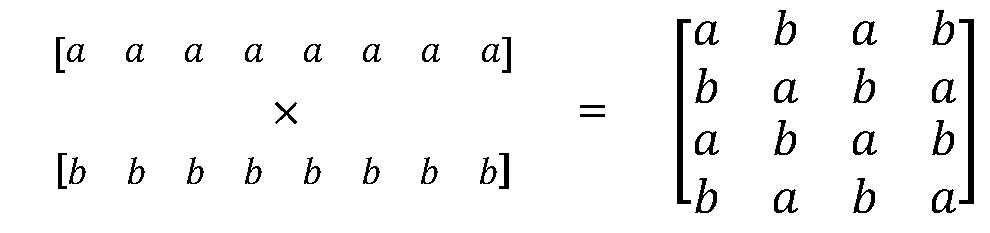
\includegraphics[width=0.8\textwidth]{pic/cross_conv.pdf}}
  \caption{棋盘式特征重组}
  \label{cross_conv}
\end{figure}
% NATLP采用卷积神经网络来完成邻居信息的构造,利用特定关系参数生成网络来为不同关系生成对应的卷积神经网络参数。为了显示的捕捉不同关系之间的共性,NATLP引入了一个全局关系嵌入参与网络参数的生成。

具体的,给定一个邻居实体$e$和相连的关系$r$,模型先采用棋盘式特征重组的方式将实体嵌入和关系嵌入重塑为二维张量:
\begin{equation}
  \phi_{chk}\left(\boldsymbol{e},\boldsymbol{r}\right) 
\end{equation}
其中$\phi_{chk}$代表棋盘式特征重组,$\boldsymbol{e} \in \mathbb{R} ^d$为实体$e$的嵌入表示,$\boldsymbol{r} \in \mathbb{R}^d$为关系$r$的嵌入表示,$d$为嵌入的维度。

将实体和关系嵌入表示重塑为二维张量之后,NATLP会对其进行循环卷积操作:
\begin{equation}
  \phi_{chk}\left(\boldsymbol{e},\boldsymbol{r}\right) \circledast \omega_r
\end{equation}

其中$\circledast$代表循环卷积。相比于普通的卷积操作,循环卷积能够捕捉更多的特征交互。卷积完成后,NATLP将卷积的输出重组为一维向量,再经过线性变化之后就可以得到邻居实体向中心实体传递的信息$m_{e,r} \in \mathbb{R} ^d$:
\begin{equation}
  m_{e,r}=f\left(vec\left(f\left(\phi_{chk}\left(\boldsymbol{e},\boldsymbol{r}\right) \circledast \omega_r \right)\right)\mathbf{W}_r\right)
\end{equation}
其中$f(\cdot )$代表ReLU激活函数,$vec(\cdot)$代表将卷积的输出重整为一维向量的操作。

为了让模型能够充分捕获关系对于实体消息传递的影响,NATLP采用参数生成网络来为卷积层和全连接层生成关系对应的特定参数$\omega_r$和$\mathbf{W}_r$。同时,为了显示地捕捉不同关系之间的共性,NATLP引入了一个全局关系嵌入$\boldsymbol{r}_{global}$参与网络参数的生成:
\begin{gather}
  \omega_r = \mbox{Re3D}\left(\mathbf{M}_{conv}\left[\boldsymbol{r};\boldsymbol{r}_{global}\right]\right) \\
  \mathbf{W}_r = \mbox{Re2D}\left(\mathbf{M}_{fc}\left[\boldsymbol{r};\boldsymbol{r}_{global}\right]\right)
\end{gather}

其中$\mathbf{M}_{conv} \in \mathcal{R}^{n_{conv}\times k_{size} \times k_{size} \times d}$为卷积层参数生成网络,$n_{conv}$为卷积核的数量,$k_{size}$为卷积核的边长,$\mathbf{M}_{fc}$为全连接层参数生成网络,$\mbox{Re3D}(\cdot)$和$\mbox{Re2D}(\cdot)$代表将参数生成网络的输出重整为卷积层和全连接层参数需要的三维张量和二维张量的形式。$\boldsymbol{r}_{global}$为全局关系嵌入。通过全局关系嵌入$\boldsymbol{r}_{global}$,模型能够捕捉到不同关系之间的共同特征,当部分关系种类训练数据较少时,模型通过全局关系嵌入也能获得不错的泛化能力。